 \documentclass[]{article}

% Use utf-8 encoding for foreign characters
\usepackage[utf8]{inputenc}

% Setup for fullpage use
\usepackage{fullpage}
\usepackage{graphicx}

\usepackage[francais]{babel}

\usepackage{times}
%\usepackage{rotate}
%\usepackage{lscape}

\usepackage{color}
\usepackage{needspace}
\usepackage{float}

\newcommand{\placeholder}[1]{{\noindent \color{red}[ #1 ]}}

\begin{document}

%\frontmatter          % for the preliminaries
%\pagestyle{headings}  % switches on printing of running heads
%\mainmatter              % start of the contributions

\title{
{\Huge Rapport de Modélisation}\\
Projet de Génie Logiciel\\
\smallskip
{\small Activité d'Apprentissage \textsf{S-INFO-015}}\\
}

\author{Groupe numéro: 3\\
Membres du groupe:\\
\textbf{DOM Eduardo , DHEUR Victor, AMEZIAN Aziz}\\
}


\date{Année Académique : 2017 - 2018\\
BAC 2 en Sciences Informatiques\\
\vspace{1cm}
Faculté des Sciences, Université de Mons}

\maketitle              % typeset the title of the contribution

\bigskip
\begin{center} \today \end{center}

\newpage
%%%%%%%%%%%%%%%%%%%%%%%%%%%%%%%%%%%%%%%%%%%%%%%%
%%%%%%%%%%%%%%%%%%%%%%%%%%%%%%%%%%%%%%%%%%%%%%%%
\section{Introduction}\label{sec:intro}

Ce document contient les différents diagrammes que nous avons créés afin de modéliser notre projet. Une explication expliquant ce que ces diagrammes représentent est fournie avec chaque diagramme.

\section{Diagrammes}

\subsection{Diagrammes de cas d'utilisation}

Ce diagramme d'utilisation montre à quelles fonctionnalités l'utilisateur a accès en utilisant notre application.

\begin{figure}[H]
\begin{center}
  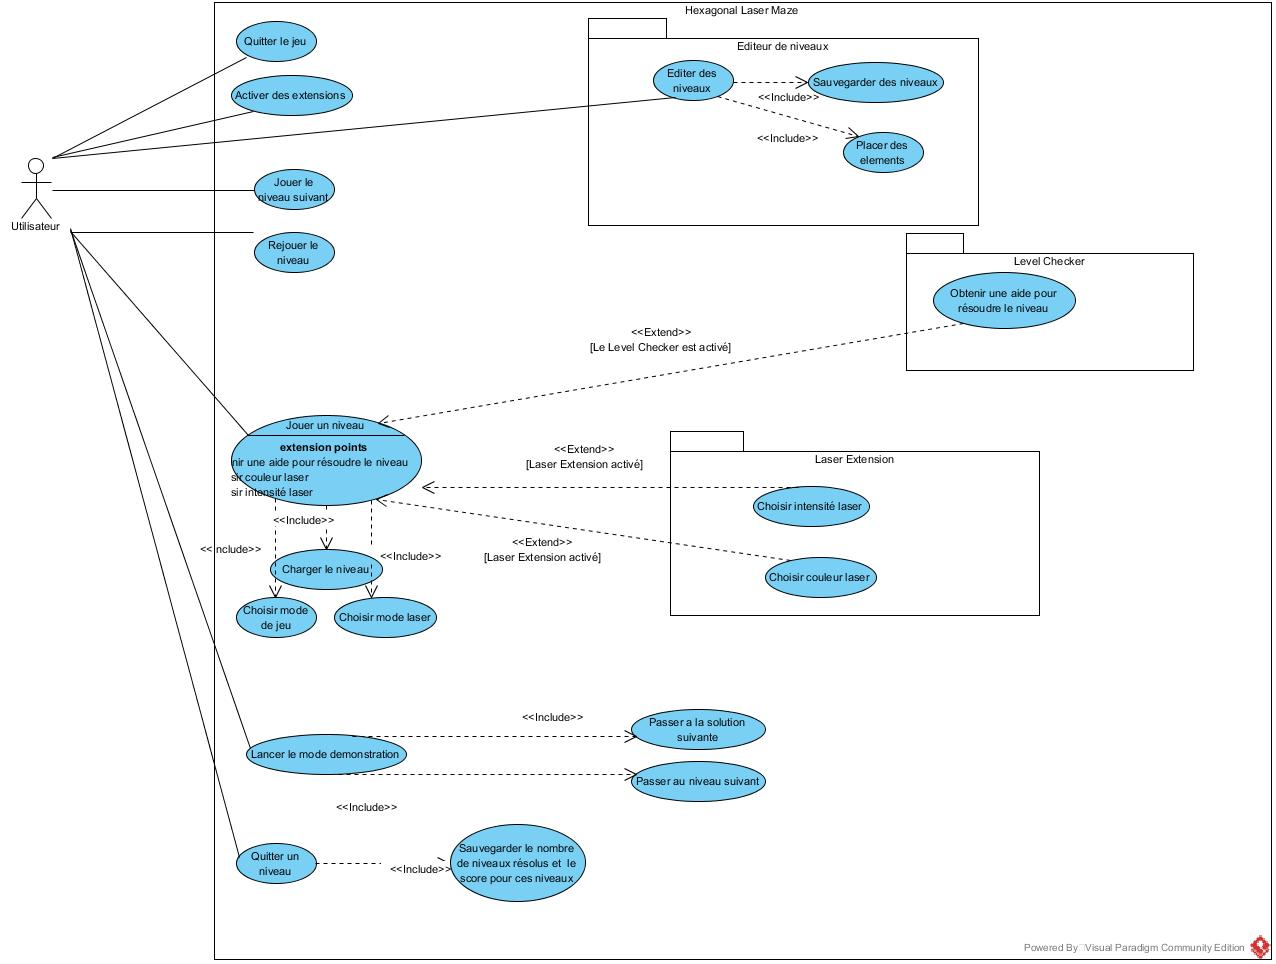
\includegraphics[width=\textwidth]{UseCase1.jpg}
  \caption{Diagramme de cas d'utilisation}\label{fig:auto}
\end{center}
\end{figure}

\subsection{Diagrammes de classes}

Nous avons choisi de séparer le modèle, la vue et le contrôleur dans 3 packages distincts. Un package supplémentaire s'occupe des classes utilitaires. Le modèle s'occupe de la logique du jeu. La vue gère uniquement l'affichage du modèle. Le contrôleur s'occupe de recevoir les entrées extérieures et de les communiquer au modèle et à la vue. Une classe peut ensuite combiner ces 3 éléments pour organiser le jeu. La classe \emph{Game} s'occupe de représenter une partie jouée. La classe \emph{GameEditor} représente le jeu vu de l'éditeur. Enfin, la classe \emph{AutomaticGame} représente le jeu en mode démonstration.

Séparer le modèle, la vue et le contrôleur peut nous aider à mieux organiser le projet et nous apporte 2 avantages. La premier est que cela nous permet de redéfinir séparément ces 3 éléments si cela est nécessaire. Par exemple, l'éditeur peut disposer d'un contrôleur spécifique. Deuxièmement cela permet d'éviter le couplage. Ainsi, la classe \emph{LevelChecker} a uniquement besoin d'être liée au modèle pour trouver la solution d'un niveau.

Nous avons principalement détaillé les classes de notre modèle. L'objet \emph{Map} en est l'objet central. Il contient un tableau d'objets \emph{Hexagon}, une référence vers chaque source et une liste d'objets \emph{Segment} permettant au \emph{MapRenderer} de dessiner le laser.

Pour donner une position à chaque hexagone, nous avons choisi d'utiliser le système "offset coordinates" avec "vertical layout" car c'est le système que LibGDX utilise. De plus, il ne rend pas les calculs beaucoup plus complexe par rapport à nos besoins.
L'objet \emph{Edge} du package \emph{util} nous permet de désigner un côté spécifique d'un hexagone. Il est convertible en \emph{int} pour nous aider à faire certains calculs.

Pour chaque type d'hexagone différent, une spécialisation de \emph{Hexagon} a été créée. Cela nous permet de définir pour chaque hexagone le comportement qu'il doit adopter si un laser le traverse en arrivant par un certain côté et avec un certain laser. La méthode \emph{traverse} permet de notifier à l'hexagone qu'il a été traversé et de modifier le laser en fonction de l'hexagone. Si l'hexagone possède un modifier, celui-ci est aussi traversé. On peut utiliser \emph{traverseBack} pour annuler cet effet. La méthode \emph{containsLaser} indique si l'on va croiser un laser de façon à perdre en traversant l'hexagone d'un certain côté avec un certain laser. La méthode \emph{getNextEdges} donne les côtés par lesquels va sortir le laser s'il entre par un certain côté, sans tenir compte du fait que la laser pourrait en croiser un autre. Chaque hexagone implémentera donc cette méthode en faisant des calcules spécifiques pour déterminer quels seront les côtés de sortie du laser. Pour terminer, \emph{getNextHexagon} renvoie l'hexagone adjacent par rapport à un certain côté.

Chaque objet \emph{Source} contient un objet Laser définissant la couleur et l'intensité du laser partant de cette source. Cet objet est ensuite utilisé de manière à maintenir la couleur et l'intensité actuelles du laser lorsque l'on traverse les hexagones.

\begin{figure}[H]
\begin{center}
  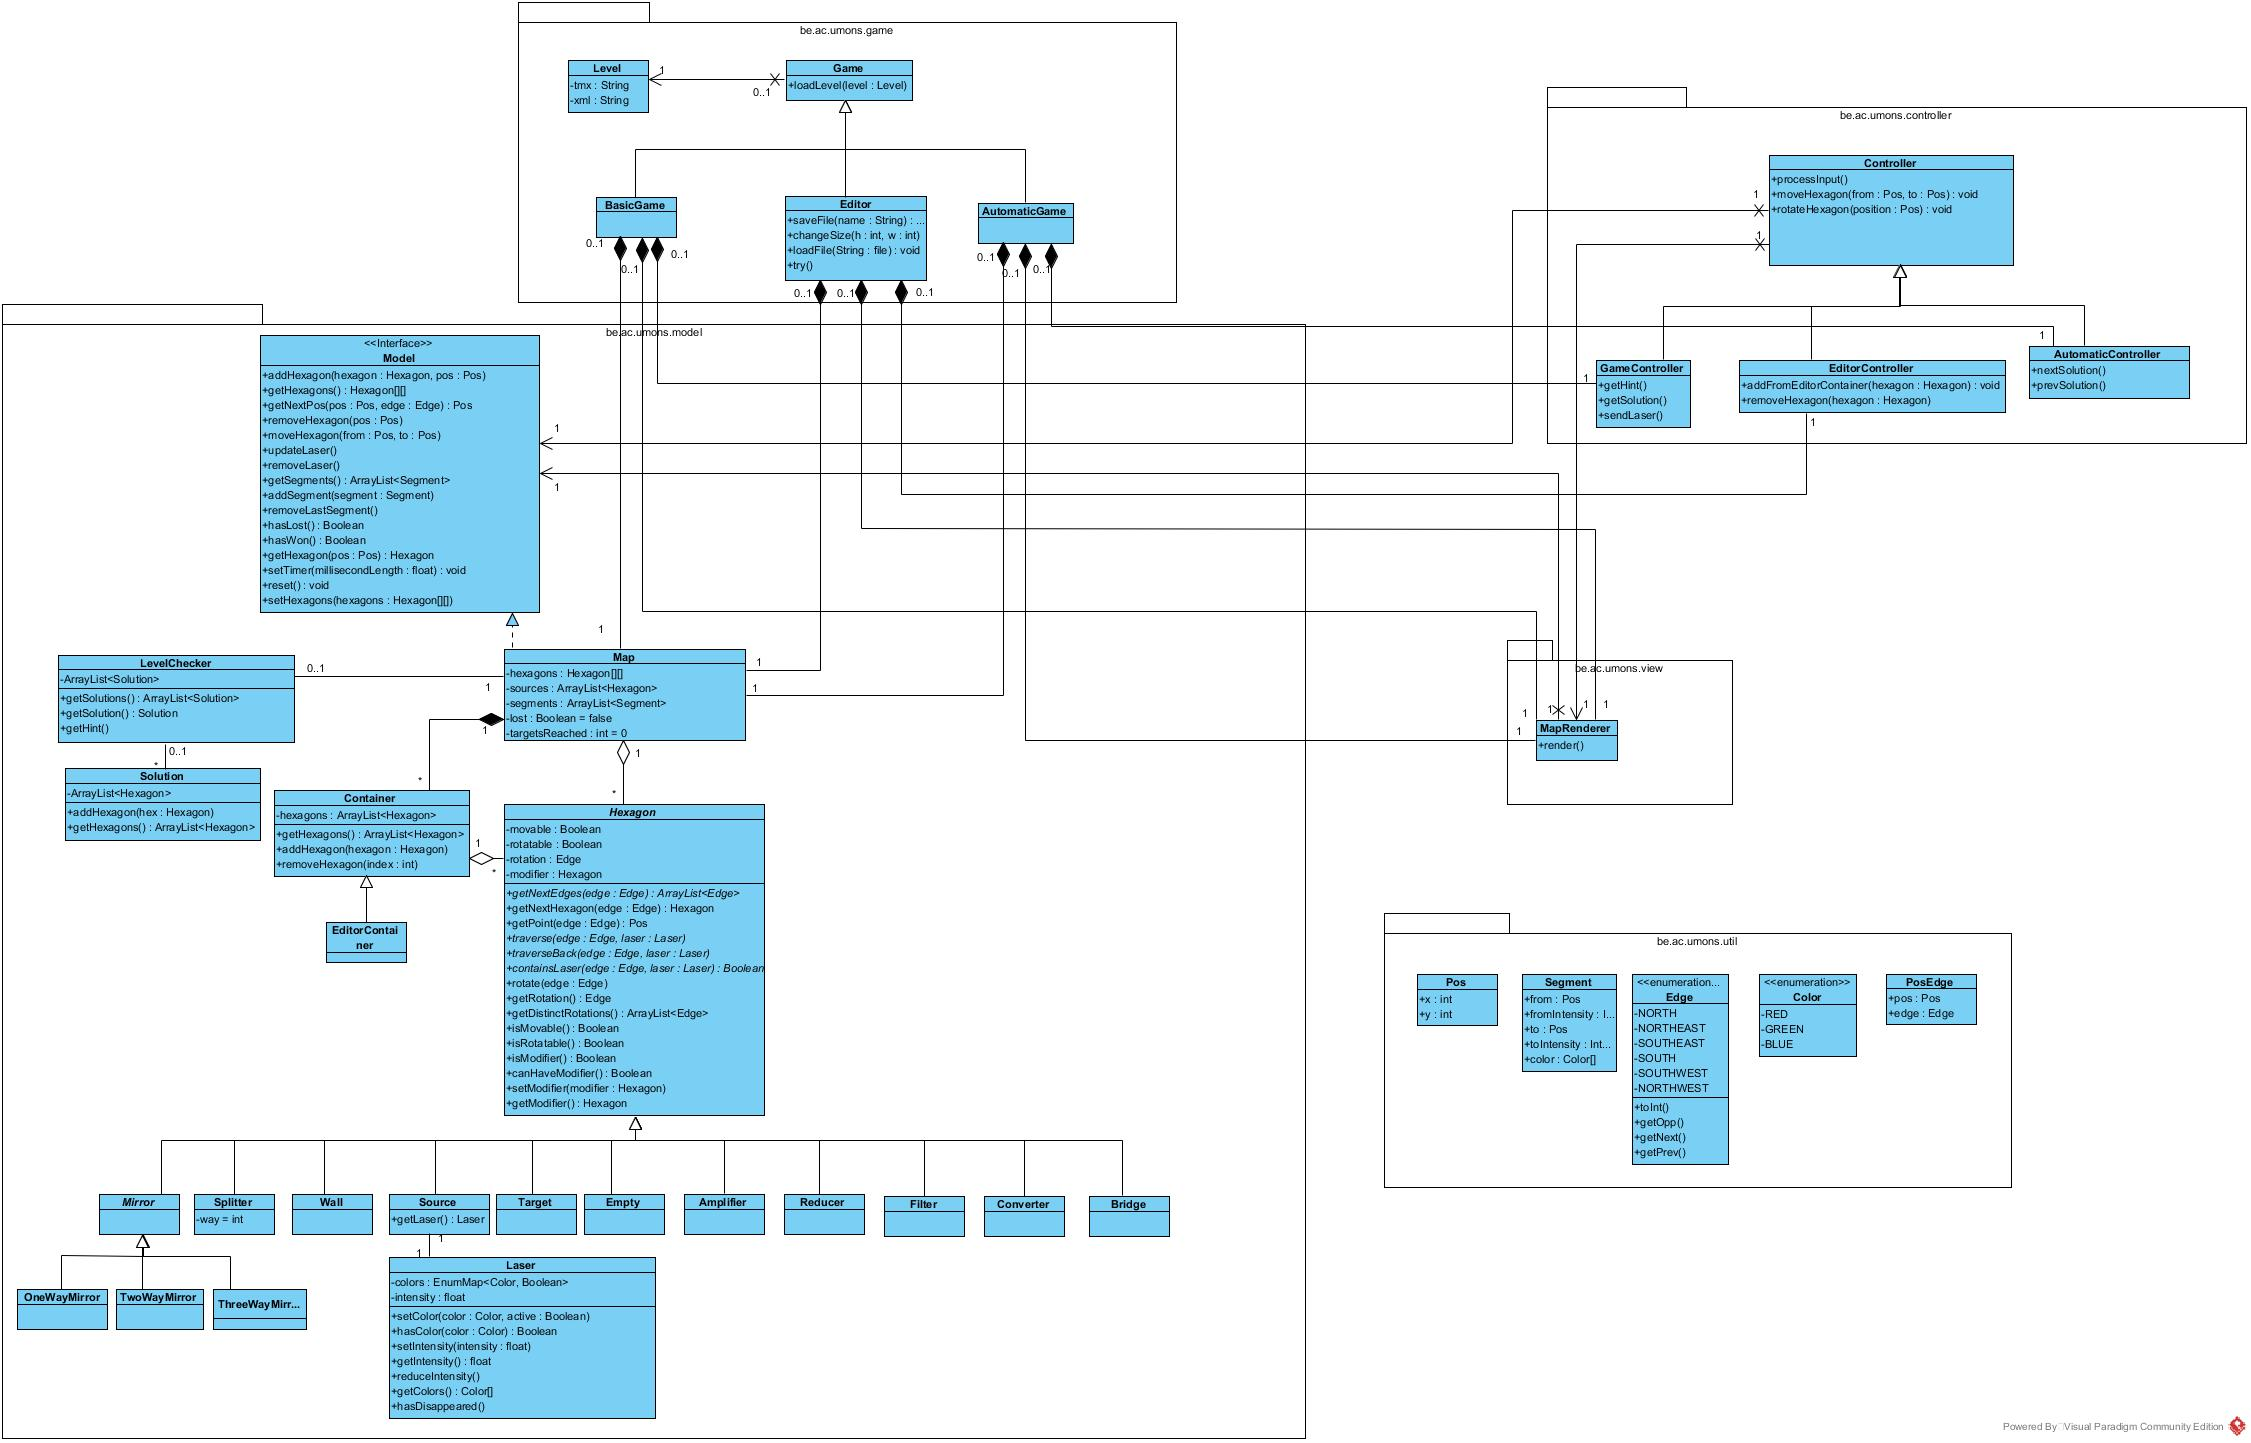
\includegraphics[width=\textwidth]{Class1.jpg}
  \caption{Diagramme de classe}\label{fig:auto}
\end{center}
\end{figure}

\subsection{Diagrammes d'états}

Les diagrammes d'états suivants indiquent comment l'utilisateur peut se déplacer dans l'application, généralement à l'aide d'événements générés par des clics de souris. Ces etats et événements ont été nommes en nous basant sur les éléments présents dans notre maquette d'interface d'utilisateur.

Le premier diagramme montre les déplacements que l'utilisateur pourra effectuer pour se déplacer entre les différents menus. Une fois que celui-ci entre dans l'état \emph{Game}, \emph{Editor} ou \emph{Automatic Game}, celui-ci peut naviguer entre différents sous-états, en fonction de son interaction avec l'interface de jeu. Par exemple, en cliquant sur un hexagone, l'utilisateur peut entrer dans un nouveau sous-état(\emph{Hexagon Clicked}) lui permettant de faire pivoter les hexagones. Dans ces diagrammes ont distingue trois types d'hexagones :
\begin{enumerate}
\item \emph{Hexagon} : Les hexagones présents sur le plateau de jeu.
\item \emph{Available Hexagon} : Les hexagones a disposition de l'utilisateur pour résoudre le niveau.
\item \emph{New Hexagon} : Les Hexagons a disposition de l'utilisateur pour modifier des niveaux dans l'editeur de niveaux.
\end{enumerate}

\begin{figure}[H]
\begin{center}
  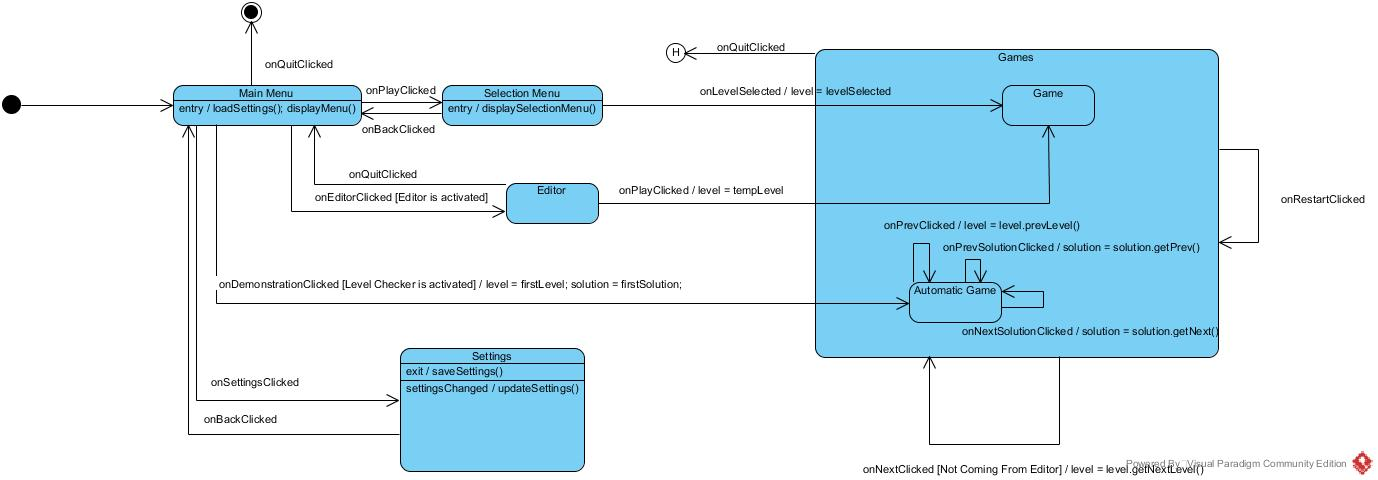
\includegraphics[width=\textwidth]{State1.jpg}
  \caption{Diagramme d'état représentant la navigation entre les menus}\label{fig:auto}
\end{center}
\end{figure}

\begin{figure}[H]
\begin{center}
  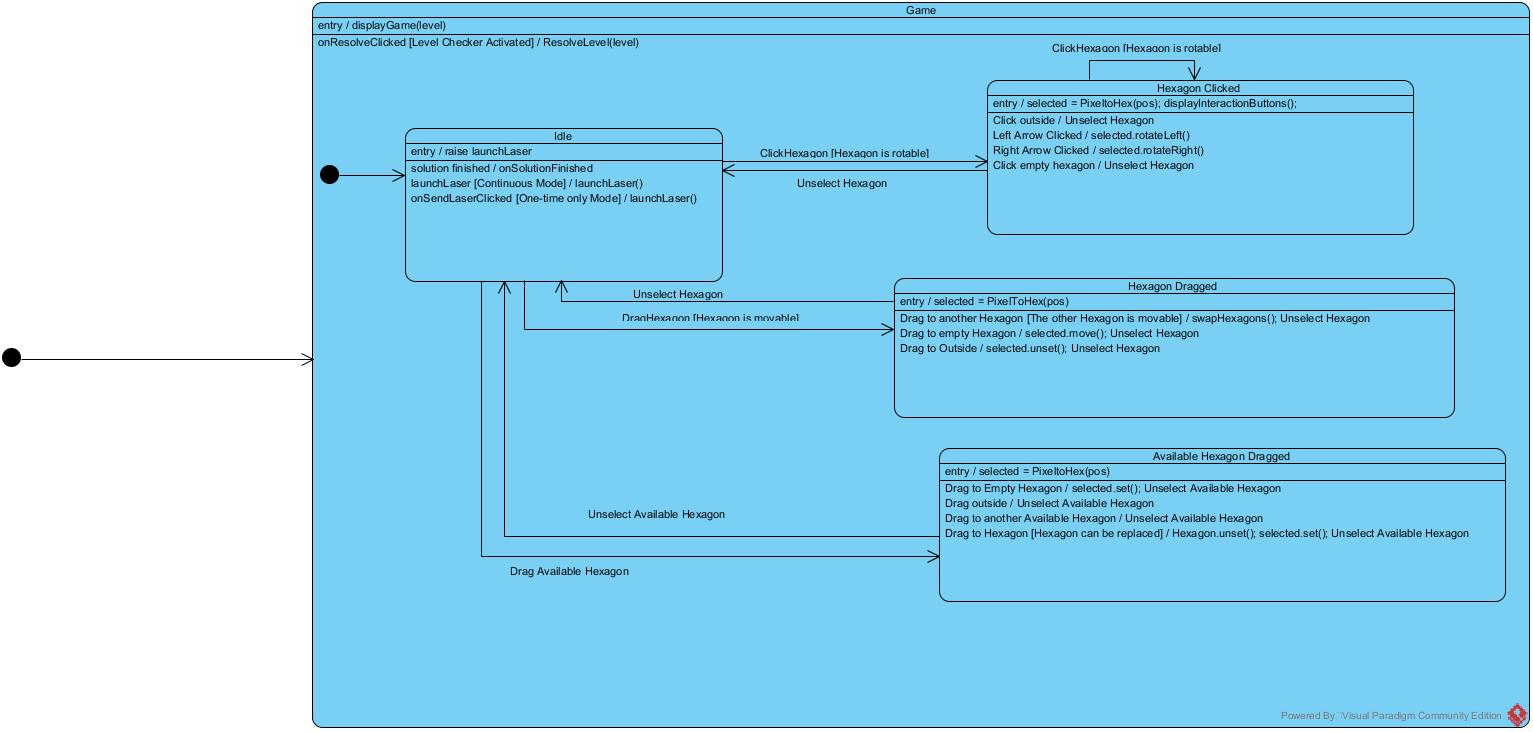
\includegraphics[width=\textwidth]{State2.jpg}
  \caption{Diagramme d'état représentant les sous-états de Game}\label{fig:auto}
\end{center}
\end{figure}

\begin{figure}[H]
\begin{center}
  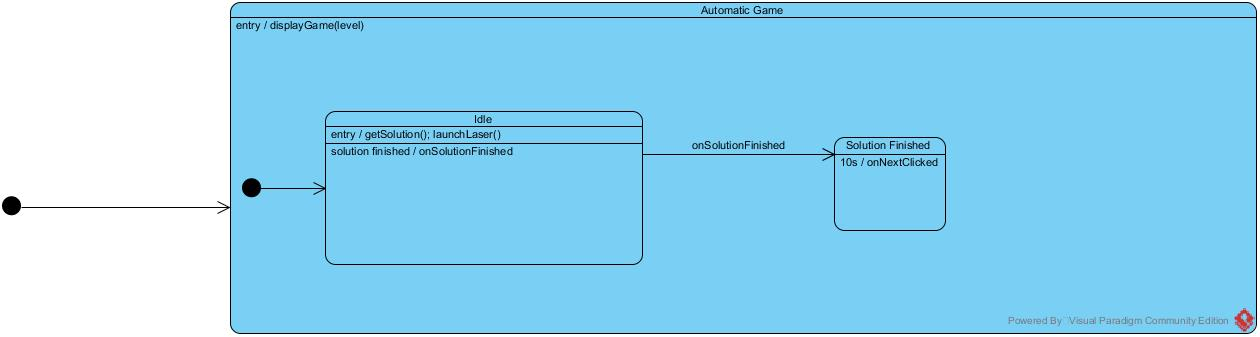
\includegraphics[width=\textwidth]{State3.jpg}
  \caption{Diagramme d'état représentant les sous-états de Automatic Game}\label{fig:auto}
\end{center}
\end{figure}

\begin{figure}[H]
\begin{center}
  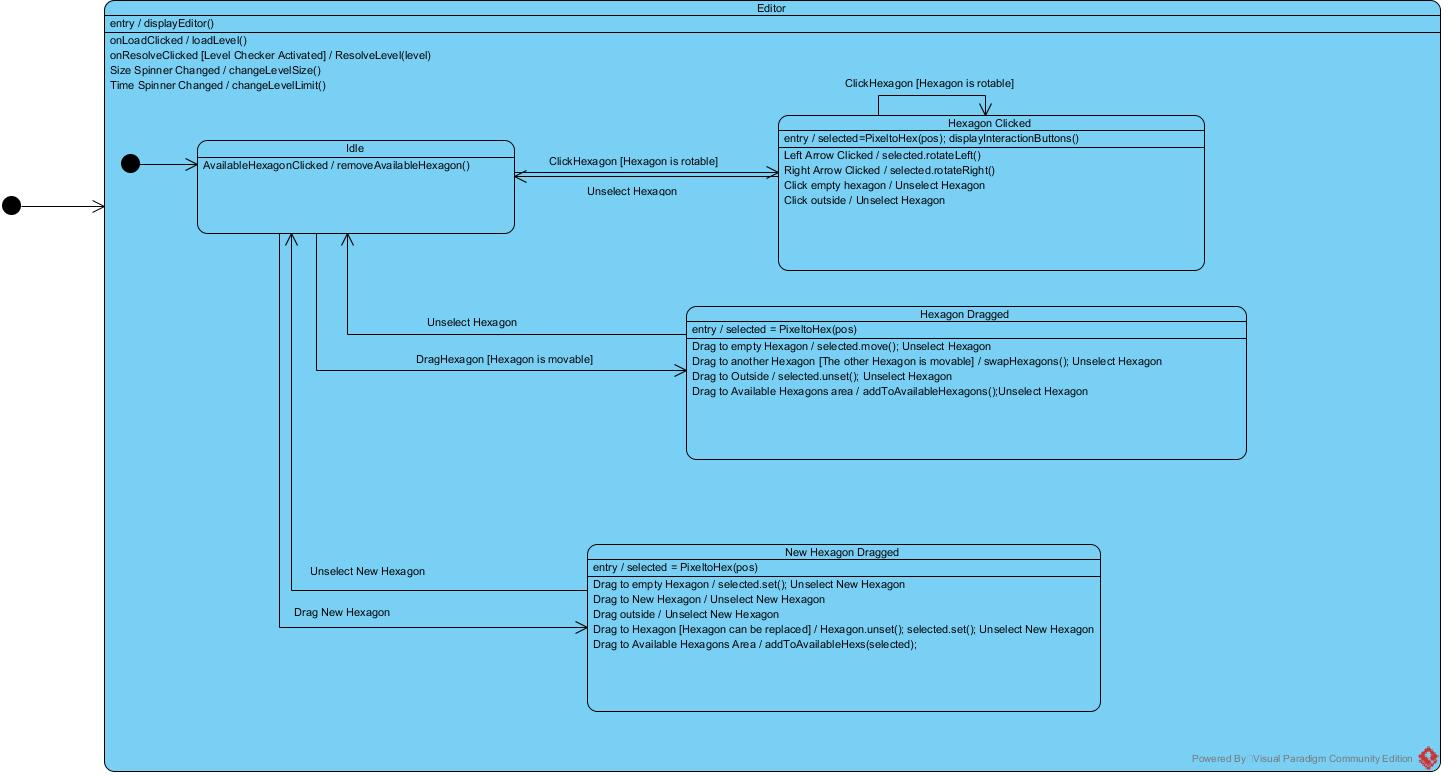
\includegraphics[width=\textwidth]{State4.jpg}
  \caption{Diagramme d'état représentant les sous-états de Editor}\label{fig:auto}
\end{center}
\end{figure}

\subsection{Diagrammes d'activités}

Les 3 premiers diagrammes d'activité montrent comment le laser est envoyé pour finalement détecter si le joueur a éventuellement gagné ou perdu. Ils indiquent aussi comment les objets \emph{Segment} représentant le laser sont créés.

Le dernier diagramme représente les actions effectuées lorsqu'un utilisateur place un nouvel hexagone sur un hexagone existant.

\begin{figure}[H]
\begin{center}
  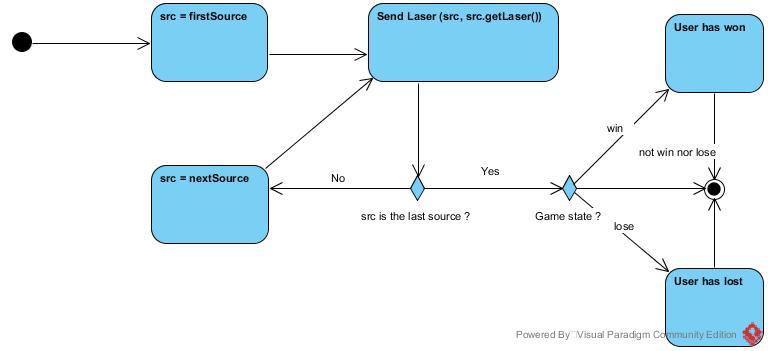
\includegraphics[width=\textwidth]{Activity1.jpg}
  \caption{Diagramme d'activité représentant la détection de victoire et défaite}\label{fig:auto}
\end{center}
\end{figure}

\begin{figure}[H]
\begin{center}
  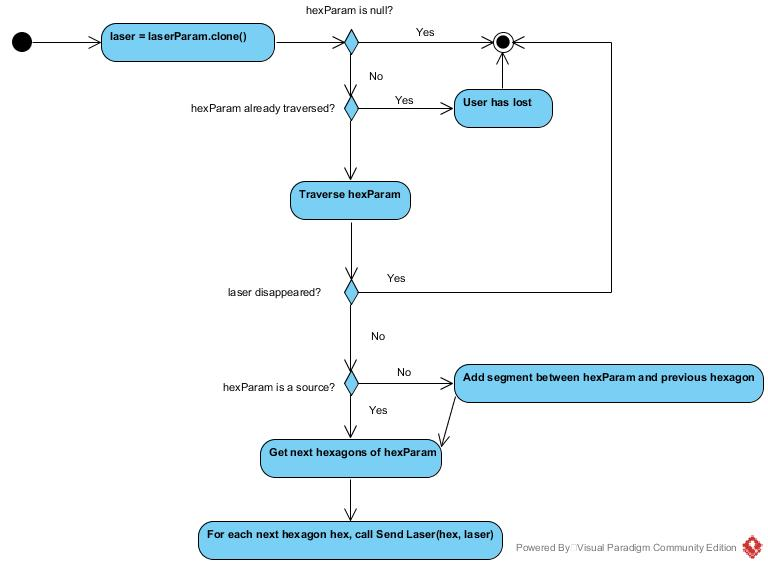
\includegraphics[width=\textwidth]{Activity2.jpg}
  \caption{Diagramme d'activité représentant la transmission du laser}\label{fig:auto}
\end{center}
\end{figure}

\begin{figure}[H]
\begin{center}
  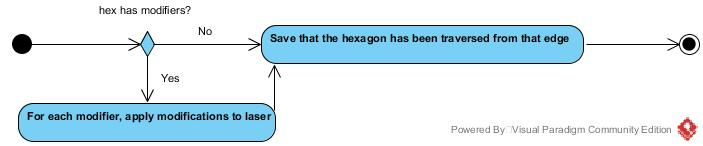
\includegraphics[width=\textwidth]{Activity3.jpg}
  \caption{Diagramme d'activité représentant la fait de traverser un hexagone}\label{fig:auto}
\end{center}
\end{figure}

\begin{figure}[H]
\begin{center}
  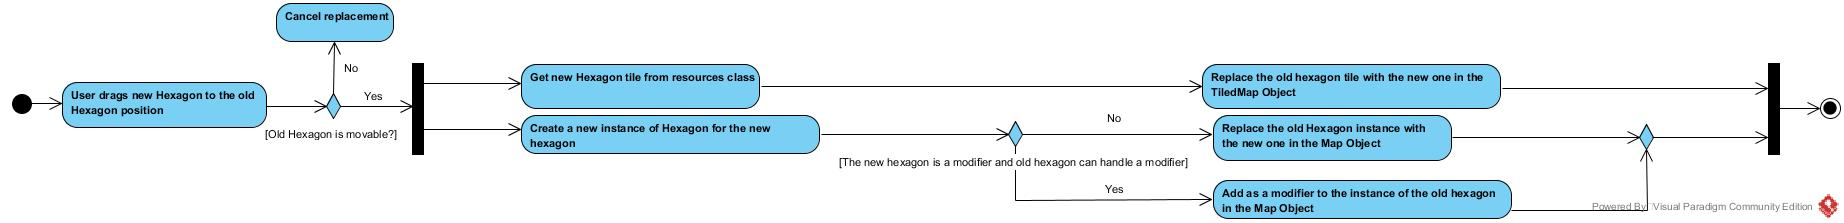
\includegraphics[width=\textwidth]{Activity4.jpg}
  \caption{Diagramme d'activité représentant le remplacement d'un hexagone}\label{fig:auto}
\end{center}
\end{figure}

\subsection{Diagrammes de séquences}

\subsubsection{Game Flow}

Ce diagramme montre les différentes interactions entre les objets principaux lors du déroulement d'une partie. Basiquement, lorque l'objet \emph{Game} est créé, celui-ci s'occupe de créer le modèle, la vue et le contrôleur. Ensuite, dans une boucle infinie générée par \emph{LibGDX}, le \emph{GameController} s'occupe de prendre les entrées extérieures (souris principalement) et le \emph{MapRenderer} s'occupe de dessiner la \emph{Map} à chaque itération.

\begin{figure}[H]
\begin{center}
  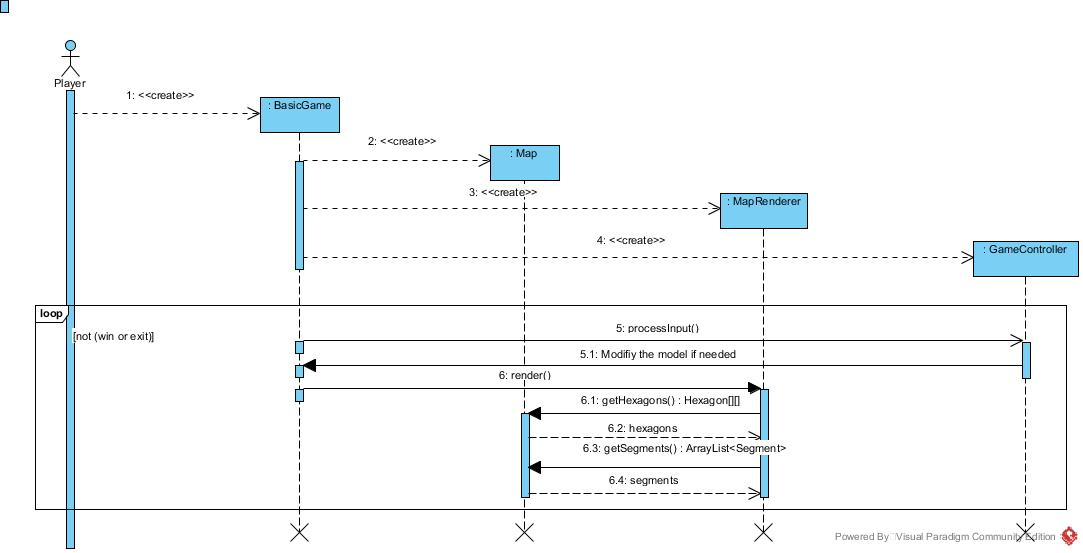
\includegraphics[width=\textwidth]{Sequence1.jpg}
  \caption{Diagramme de séquence représentant le déroulement d'un partie}\label{fig:auto}
\end{center}
\end{figure}

\subsubsection{Level Checker}

Les 3 diagrammes suivants représentent le fonctionnement du Level Checker. Celui-ci va communiquer uniquement avec le modèle afin de générer les solutions correspondant au modèle. Une explication du fonctionnement de cet algorithme est fournie ici. Les objets non déplaçables sont considérés déjà placés sur la \emph{Map}, tandis que les autres sont dans l'objet \emph{Container} de la \emph{Map}.

J'ai cherché à trouver un algorithme qui pouvait donner toutes les solutions distinctes, et cela de manière efficace.
Une première idée aurait été d'utiliser une technique de brute-force, mais cela aurait été bien trop lent.
C'est pourquoi je suis parti de l'idée que chaque bloc "utile" à la solution doit se trouver sur le chemin des lasers, ce qui limite énormément les possibilités.
Toute solution est en fait constituée de blocs placés dans un certain ordre le long des lasers.
Les sources doivent elles être placées par brute-force (si elles sont déplaçables ou orientables) étant donné que nous n'avons pas d'indice sur leur position et direction, tout en faisant attention à éviter les duplications de configurations.
Afin de représenter tous les ordres possibles de blocs sans répéter les solutions, il suffit de générer toutes les permutations distinctes possibles des objets à placer.

Le premier diagramme de séquence montre donc comment les sources déplaçables sont placées (les sources non déplaçables étant considérées déjà placées). Une fois que toutes les sources sont placées, pour chaque permutation des objets présents dans le conteneur, on entre dans le deuxième diagramme.

Ce diagramme montre comment les objets sont placés dans chaque récursion. Pour effectuer les récursions, j'ai choisi de maintenir une liste d'objets \emph{PosEdge} nommée \emph{laserSources} représentant la dernière position et orientation de chaque laser devant encore être calculé. Elle est initialisée avec  Cela permet à l'algorithme de savoir quels lasers il lui reste à traiter. En supprimant des éléments de \emph{laserSources} ou en en ajoutant, l'algorithme peut gérer le cas où le laser s'arrête, et le cas où celui-ci se divise (splitter), et continuer avec les autres éléments jusqu'à ce qu'il n'en reste plus. Cela peut être géré de manière à ce que chaque récursion ne prenne qu'une complexité O(1).

A chaque récursion, la première étape va donc être de vérifier qu'il reste des \emph{laserSource} à traiter. Si non, tous les lasers ont été créés et il ne reste qu'à vérifier si on a gagné.

Ensuite, un élément représentant le laser qu'on traite actuellement est enlevé de \emph{laserSources}. On sauvegarde aussi l'objet actuel à cette position.

Si l'objet actuel n'existe pas, on continue simplement avec les autres éléments de laserSources. Si on croise un autre laser, inutile de continuer les récursions car on sait que l'on a perdu. Sinon, 2 possibilités de placement se présentent.
\begin{itemize}
\item Soit on place le prochain hexagone de la permutation (dans chaque orientation distincte s'il est orientable) à condition que l'objet actuel est un hexagone vide.
En effet, s'il n'est pas un hexagone vide, cet hexagone ne peut qu'être un objet non-déplaçable qui était déjà présent à cette position
ou un objet que nous avons déjà placé dans une récursion précédente, et qui ne devrait pas être remplacé.
Après avoir placé cet objet, on doit passer au prochain objet de la permutation.
\item Soit on laisse le bloc actuel.
\end{itemize}
Pour ces 2 possibilités de placement, on doit tester chaque orientation possible de l'hexagone, calculer les prochain côtés atteints par l'hexagone, mettre à jour \emph{laserSources} selon ces côtés et notifier  l'objet qu'on la traversé.
Ensuite, après chaque récursion, il convient d'annuler ce qui a été fait avant pour tester chaque possibilité de placement des hexagones le long des lasers indépendamment l'une de l'autre.
C'est ce que représente le 3ème diagramme de séquence.

Evidemment, cet algorithme pourrait ne pas être assez rapide, notamment si :
\begin{itemize}
\item Parmi les objets à placer, de nombreux sont distincts.
\item Il y a beaucoup d'espace libre, ce qui laisserait beaucoup de possibilités de lasers.
\item Plusieurs sources doivent être placées.
\end{itemize}

Une autre possiblité d'optimisation que je pourrais appliquer est de calculer le nombre de lasers possibles, en fonction du nombre de sources et splitters.
Ce nombre moins le nombre de targets donnerait le nombre maximal de lasers que l'on peut arrêter afin d'avoir une chance de gagner.
Cela permettrait de limiter les récursions, en arrêtant l'algorithme si trop de lasers ont été bloqués.

\begin{figure}[H]
\begin{center}
  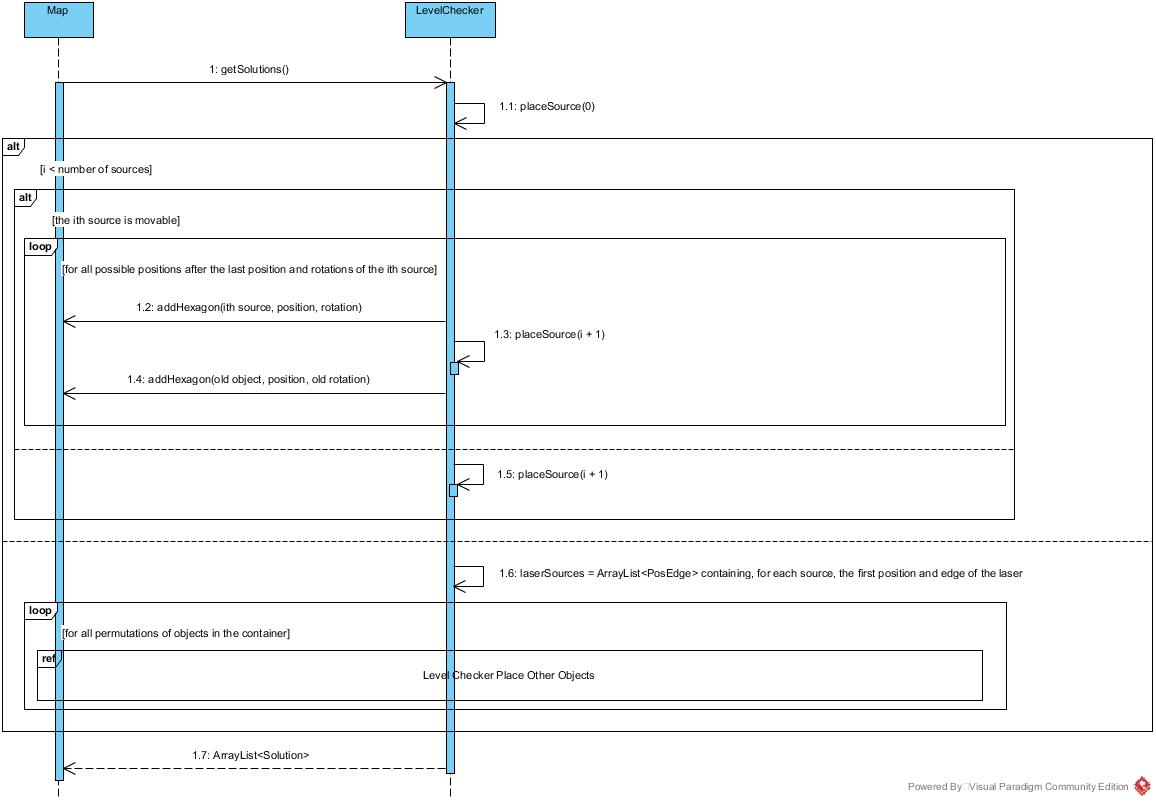
\includegraphics[width=\textwidth]{Sequence2.jpg}
  \caption{Diagramme de séquence représentant le placement des sources lors de la résolution d'un niveau}\label{fig:auto}
\end{center}
\end{figure}

\begin{figure}[H]
\begin{center}
  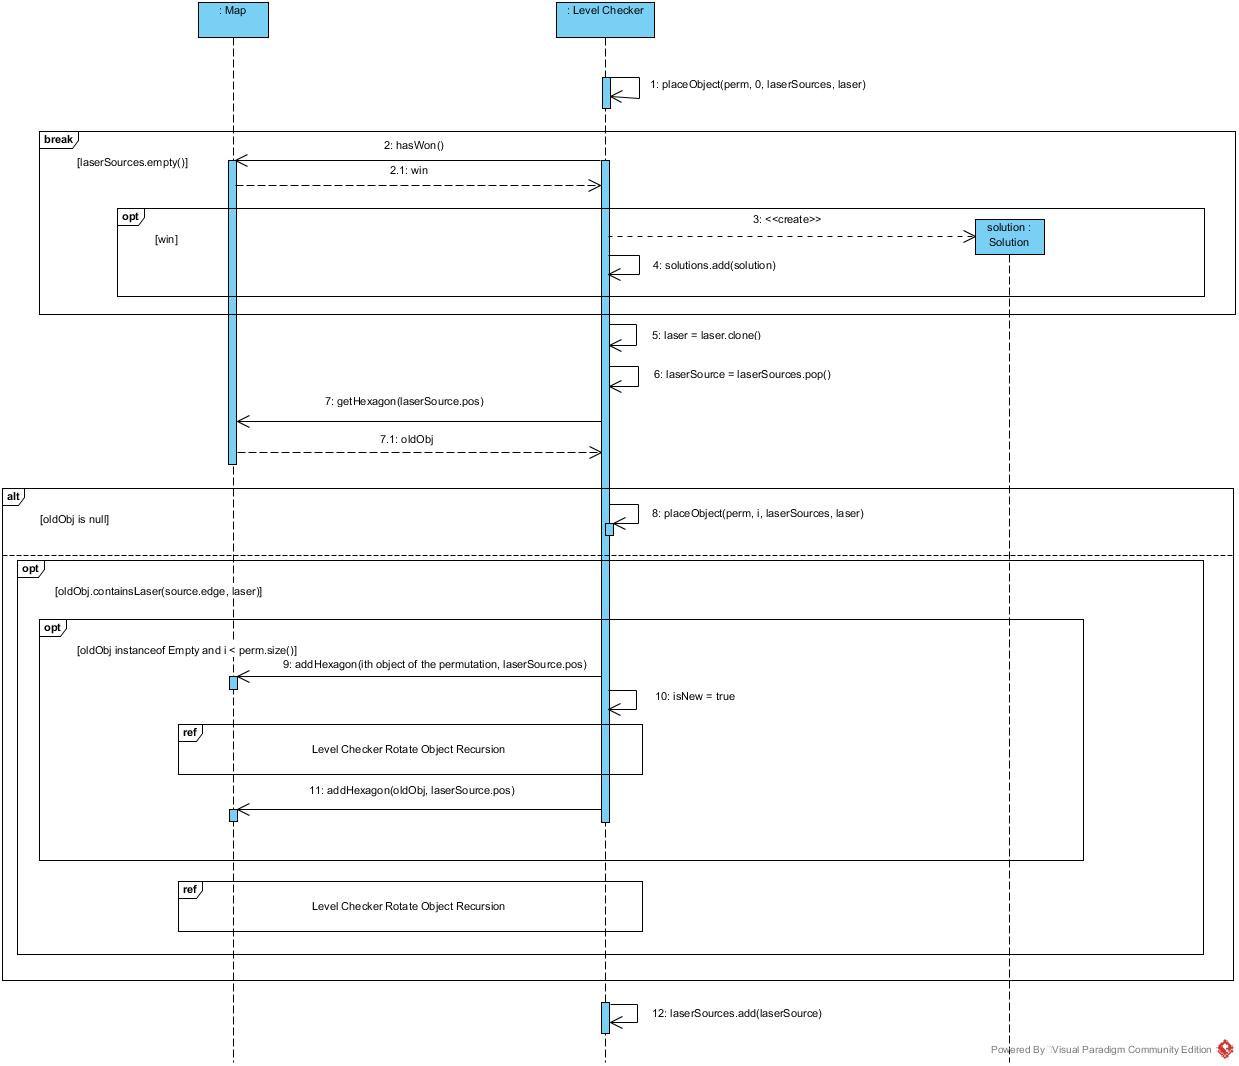
\includegraphics[width=\textwidth]{Sequence3.jpg}
  \caption{Diagramme de séquence représentant le placement des objets autres que sources lors de la résolution d'un niveau}\label{fig:auto}
\end{center}
\end{figure}

\begin{figure}[H]
\begin{center}
  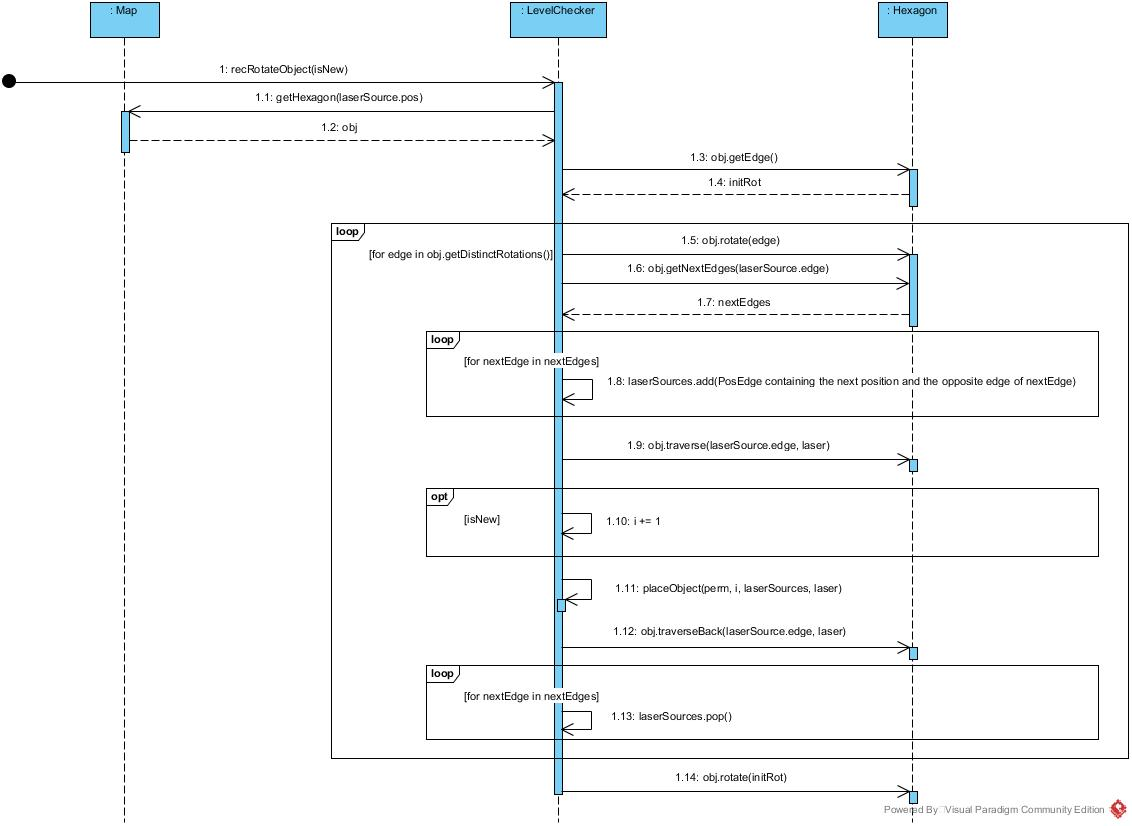
\includegraphics[width=\textwidth]{Sequence4.jpg}
  \caption{Diagramme de séquence représentant le placement d'un objet dans chaque orientation lors de la résolution d'un niveau}\label{fig:auto}
\end{center}
\end{figure}

\end{document}
